\makeatletter
% \tikzoption{canvas is plane}[]{\@setOxy#1}
% \def\@setOxy O(#1,#2,#3)x(#4,#5,#6)y(#7,#8,#9)%
%   {\def\tikz@plane@origin{\pgfpointxyz{#1}{#2}{#3}}%
%    \def\tikz@plane@x{\pgfpointxyz{#4}{#5}{#6}}%
%    \def\tikz@plane@y{\pgfpointxyz{#7}{#8}{#9}}%
%    \tikz@canvas@is@plane
%   }
% \makeatother 


%y={(-1cm,0.5cm)},x={(1cm,0.5cm)}, z={(0cm,1cm)}
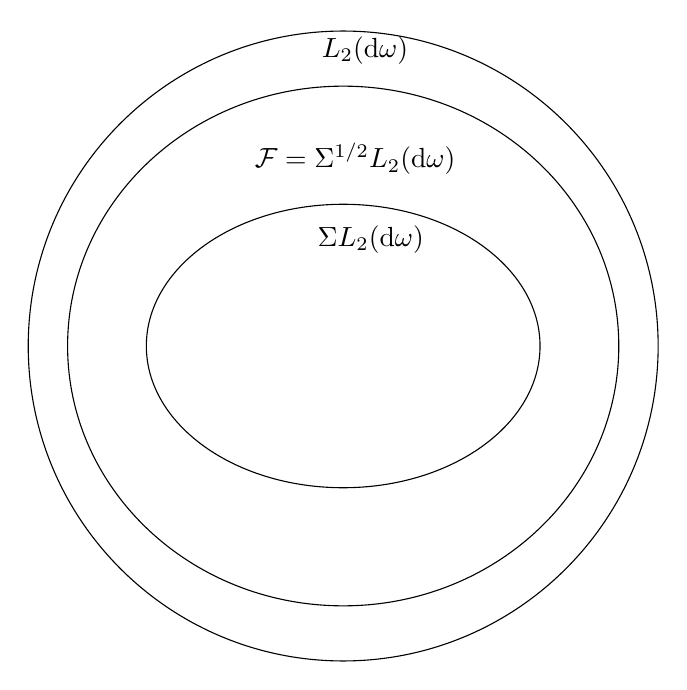
\begin{tikzpicture}[]
\coordinate (A) at (1.4,1,0);
\coordinate (B) at (6.7,1,0);
\coordinate (B2) at (4.1,1,0);
\coordinate (C) at (6.7,-3,0);
\coordinate (D) at (8,-0.3,0);
\coordinate (E) at (8,-1.7,0);

\coordinate (F) at (4,-1,0);


\draw (0,1) circle (4cm);

\draw (0,1) ellipse (3.5cm and 3.3cm);

%\draw (0,1) ellipse (3cm and 2.6cm);

\draw (0,1) ellipse (2.5cm and 1.8cm);


% \draw (8,1) circle (1.2cm);

% \draw (8,-3) circle (1.2cm);
% \draw[fill={rgb:red,1;white,5}] (0,0,0) -- (2,0,0) -- (2,2,0) -- (0,2,0) -- cycle;
% \draw[fill={rgb:blue,1;white,5}, opacity=0.5] (0,0,0) -- (2.2,1,0) -- (2.2,3,0) -- (0,2,0) -- cycle;

% \node[canvas is plane={O(0,2,0)x(0,1,0)y(1,2,0)}] at (0.9,-0.9) {\includegraphics[width=2.4cm, height=2.4cm]{fig/principalangles/signal_eigreconstruction_modes}};

% \node[canvas is plane={O(0,2,0)x(0,1,0)y(2.2/2.41,2+1/2.41,0)}] at (0.8,-0.6,0.1) {\includegraphics[width=2.4cm, height=2.7cm]{fig/principalangles/signal_reconstruction_principle_2}};

\begin{scope}
 %  \draw (12.2,1.8,0) node[above left = 0.5mm] {$\mathbb{B}_{\langle .,. \rangle_{\mathcal{F}}} = \bm{\Sigma}^{1/2}\mathbb{B}_{\langle .,. \rangle_{\mathrm{d}\omega}}$};
	% \draw (1.8,1.8,0) node[above left = 0.5mm] {$\mathbb{B}_{\langle .,. \rangle_{\mathrm{d}\omega}}$};
  \draw (1,4.4,0) node[above left = 0.5mm] {$\mathbb{L}_{2}(\mathrm{d}\omega$)};

  \draw (1.6,3,0) node[above left = 0.5mm] {$ \mathcal{F} = \bm{\Sigma}^{1/2}\mathbb{L}_{2}(\mathrm{d}\omega$)};
  %\draw (0.5,-2.2,0) node[above left = 0.5mm] {$\mathcal{F}$};

  % \draw (1.4,2.7,0) node[above left = 0.5mm] {$\bm{\Sigma}^{1/2+\color{red}r\color{black}}\mathbb{L}_{2}(\mathrm{d}\omega$)};

	\draw (1.2,2,0) node[above left = 0.5mm] {$\bm{\Sigma}\mathbb{L}_{2}(\mathrm{d}\omega$)};

  % \draw [->] (A) --(B2) node[above] {$\bm{\Sigma}^{1/2}$} -- (B) ;
  % \draw [->] (A) -- (F) node[above] {$\bm{\Sigma}$} -- (C) ;
  % \draw [->] (D) -- (E) ;
\end{scope}
% \begin{scope}[canvas is yz plane at x=1.25]
% \draw[fill={rgb:blue,1;white,5}] (0,0) -- (2,0) -- (2,2) -- (0,2) -- cycle;
% \end{scope}
\end{tikzpicture}
%}